% ch14a Quantum phase transitions, part a (书页 289-305 / 分册p001-017)
% 第14章 Quantum phase transitions
\chapter{量子相变}

上一章中，我们讨论了绝缘体–超导体转变与绝缘体–金属转变。由于这类转变由无序或磁场调控，热涨落不起任何作用。绝缘体–超导体型或绝缘体–金属型的相变被称为量子相变（quantum phase transition）。这类相变不像冰的熔化或液氦的 $\lambda$ 点那样通过改变温度来控制，而是通过改变某个系统参量来控制，例如缺陷的数目或载流子的浓度。在所有这些情形中，调控参量使系统在若干量子力学态之间转换，这些态要么在拓扑上看起来不同（如局域电子态与扩展电子态之间的转变），要么具有截然不同的磁性质。由于这类相变以量子力学为根基，所有量子相变都发生在绝对零度，因而受 $T=0$ 的量子临界点支配。虽然初看起来令人惊讶，但这种情况实属意料之中，因为量子力学明确地是一门关于物质的零温度理论。当然，这对化学家来说毫不意外：他们早已知道，仅通过改变化学成分，众多材料就能展现出截然不同的性质；更重要的是，这类转变会一直保持到零温。常见的例子有：仅通过化学掺杂就把层状铜氧化物（cuprate）之类的绝缘体变成超导体，或同样通过掺杂把半导体变成金属，再或通过改变 $x$ 把 $\mathrm{Li}(\mathrm{Ho},\mathrm{Tb})_x\mathrm{Y}_{1-x}\mathrm{F}_4$ 之类的铁磁体变成自旋玻璃（AR1998）。无疑，作为电子工业支柱的掺杂半导体的技术重要性早已确立。

鉴于量子相变的普遍性与重要性，关于这类现象的理论似乎应已发展得相当成熟，但实际情况并非如此。构造量子相变（QPT）理论的困难在于它们发生在零温度这一事实。所有相变都由某种类型的涨落驱动。由于热涨落在零温度下消失，QPT 必须由一种截然不同的实体驱动。在零温度下幸存下来的涨落只有量子力学起源的涨落。因此，不确定性原理处在所有 QPT 的核心。于是，在一个允许发生量子相变的微观哈密顿量中，必然存在两个描述相互竞争的有序化倾向的不对易算符。在所有量子相变中，耦合常数的大小描述了相互竞争的态之间的\emph{本质张力}（essential tension）。

横向磁场中伊辛模型的哈密顿量为这种本质张力提供了一个清晰的例子（P1979）。考虑一条自旋线性链，每个自旋都处在自旋 $z$ 分量 $S^z$ 的本征态上。近邻自旋以强度 $-J$ 发生铁磁相互作用。同时存在一个趋于使单个自旋沿 $x$ 方向排列的场。沿 $\pm x$ 轴的自旋由线性组合 $|\text{上}\rangle \pm |\text{下}\rangle$ 构成。描述该系统的哈密顿量为

\begin{figure}[H]\centering
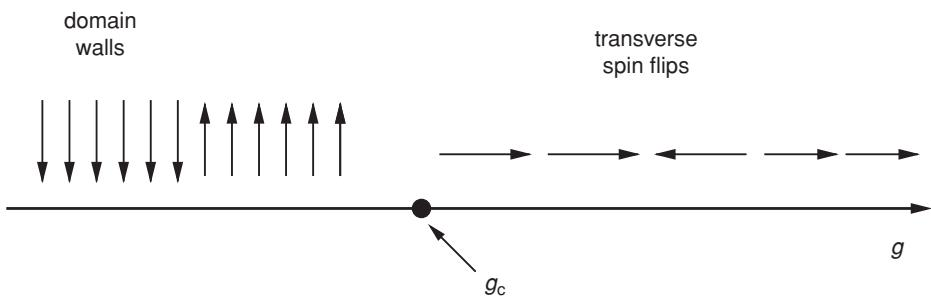
\includegraphics[width=0.7\textwidth]{figs/ch14/fig_14.1.jpg}
\caption*{图 14.1\quad 横向伊辛模型中量子相变两侧出现的局域激发。随着耦合常数 $g$ 增大，横向场的强度增大，临界点位于 $g_{\mathrm{c}}=1$。}\label{fig:auto:14.1}
\end{figure}

\begin{equation*}
H_{\mathrm{spin}} = -J \sum_j \left( g\hat{\sigma}_j^x + \hat{\sigma}_j^z \hat{\sigma}_{j+1}^z \right),\tag{14.1}
\end{equation*}

其中包含自旋横向分量与 $z$ 分量的泡利矩阵 $\hat{\sigma}_j^x$ 和 $\hat{\sigma}_j^z$。这正是相互竞争并最终决定量子临界点是否存在的两个不对易算符。这个哈密顿量虽然简单，却极为有用，因为它可以被推广（S1999）去描写磁性系统 $\mathrm{Li}(\mathrm{Ho},\mathrm{Tb})_x\mathrm{Y}_{1-x}\mathrm{F}_4$。当 $g=0$ 时，相邻自旋彼此平行排列以降低能量，整个系统于是处于总 $S^z$ 算符的一个本征态。式 (14.1) 中正比于 $g$ 的项则有利于自旋的横向取向。当 $g=\infty$ 时，所有自旋都指向 $+x$ 或 $-x$ 方向，系统从而成为 $S^x$ 的本征态。因此，$g=0$ 与 $g=\infty$ 两个极限都代表系统的定态，在其中 $\langle\hat{\sigma}^z\rangle$ 与 $\langle\hat{\sigma}^x\rangle$ 分别具有确定的取值。在这两个极限之间，系统不再处于定态，因为存在趋于破坏完美 $g=0$ 或 $g=\infty$ 序的局域激发。图 14.1 表明，在 $g=0$ 附近，局域激发由一片区域即一个畴壁构成，其中的自旋全都指向与 $g=0$ 基态中主导序相反的方向。类似地，对 $g\gg 1$，激发全都类似于局域的横向自旋翻转，这也示于图 14.1 中。鉴于 $g=0$ 与 $g=\infty$ 的基态磁性质截然不同，其准粒子激发亦然，可以想见应当在某个有限的 $g$ 值处存在一个临界点，标志着 $g=0$ 有序态的终结。事实上，这样的临界点确实存在，位于 $g=g_{\mathrm{c}}=1$，这是 Pfeuty（P1979）在一维情形下对该模型精确求解所证明的。对 $g<1$，基态在定性上类似于 $g=0$ 的铁磁体；而对 $g>1$，基态类似于 $g=\infty$ 态，所有自旋沿横向排列。耦合常数 $g$ 代表两种有序化倾向之间的本质张力，$g=g_{\mathrm{c}}=1$ 定义了量子临界点。在 $g\ll 1$ 的极限下，$\hat{\sigma}^x$ 没有确定的取值；而在相反的极端下，$\hat{\sigma}^z$ 取值的不确定度实质上为无穷大。于是，正如海森堡不确定性原理所要求的那样，自旋 $x$ 分量与 $z$ 分量不确定度的乘积在 $g$ 变化时保持恒定。由此可见，正是量子不确定性在 $g$ 被调计时驱动着相变。

在 $g_{\mathrm{c}}$ 处，基态并非特别简单。关于 $g_{\mathrm{c}}$ 处的基态我们所知道的是，它表现出标度不变性。也就是说，自旋之间的关联足够长程，以至于如果我们增大观测两个自旋所用的长度尺度，什么也不会改变。其结果是，基态波函数完全不告诉我们两个自旋相距多远。然而，可以预期这一图像在有限温度下会改变，因为准粒子的有限温度弛豫会影响问题中纯量子力学的方面。此时进入的自然时间尺度是 $\hbar/k_{\mathrm{B}}T$。因此，虽然量子相变发生在 $T=0$，只要观测的时间尺度满足一定的约束条件，相变中量子力学的那些方面在有限温度下仍可见其踪迹。支配物理关联的发散长度尺度与准粒子弛豫的时间尺度，是刻画连续量子相变的两个关键特征。事实上，正是时间尺度 $\hbar/k_{\mathrm{B}}T$ 的出现使 QPT 的理论分析变得复杂。

在本章中，我们将探讨空间维与时间维的交织如何决定量子临界点的行为。我们不分析自旋模型，而是探讨绝缘体–超导体转变的纯相位模型（phase-only model）。在该模型中，量子相变由序参量的量子力学相位的涨落支配。我们本可以同样容易地聚焦于对振幅发生涨落的模型，但纯相位模型特别富有启发性，因为它可以直接应用于约瑟夫森结阵列，而且它漂亮地阐明了不确定性原理所扮演的中心角色。我们的分析总体上是启发式的，只在必须计算之处进行计算。重点将放在驱动底层量子临界点的耦合常数所体现的本质张力上。

\section{量子转子模型}

引入绝缘体–超导体转变的纯相位模型，最简单的方式是考虑放置在二维方格子上的一组超导岛。岛上的所有电子被锁定成库珀对，并具有相同的相位。因此，纯相位模型的一个要素是对振幅在任何时刻都保持冻结。于是，我们为第 $j$ 个岛赋予一个对振幅 $\Delta$、一个确定的相位 $\theta_j$，以及一个复波函数即序参量 $\psi_j=\Delta\mathrm{e}^{\mathrm{i}\theta_j}$。此外，为简单起见，我们把库珀对当作玻色子处理。这样一个系统的能量有两项贡献：（1）每个超导岛的净能量，（2）两个岛之间的输运能量。考虑一个半径为 $R$、相对周围环境电容为 $C$ 的岛。把一个电荷为 $2e$ 的库珀对从这样的岛移到无穷远处所需的能量为 $E_{\mathrm{C}}=(2e)^2/2C$，即电容充电能。$E_{\mathrm{C}}$ 有两个重要特点。第一，$E_{\mathrm{C}}$ 按电荷的平方标度，因而必正比于 $N^2$，其中 $N$ 是岛上的库珀对总数。第二，$E_{\mathrm{C}}$ 与电容成反比。因此，当岛尺寸减小时电容项占主导。库珀对在岛 $i$ 与岛 $j$ 之间的输运要求有 $b_i^\dagger b_j$ 型的项，其中 $b_j$ 是岛 $j$ 上库珀对的湮灭算符。于是，我们的哈密顿量具有如下形式

\begin{equation*}
H = E_{\mathrm{C}} \sum_i \left( \hat{n}_i - n_0 \right)^2 - t \sum_{\langle ij\rangle} \left( b_i^\dagger b_j + b_j^\dagger b_i \right),\tag{14.2}
\end{equation*}

其中 $\hat{n}_i=b_i^\dagger b_i$ 是第 $i$ 个岛的数算符，$n_0$ 设定每个岛上的平均密度，$-t$ 是近邻岛之间的跃迁矩阵元。求和 $\langle ij\rangle$ 只限于近邻格点。式 (14.2) 被称为玻色–哈伯德模型，与第 16 章讨论的费米子对应物密切相关。式 (14.2) 具有两个不同的极限：先令动能项为零即可看出其一——在此极限下所有库珀对都被冻结在各自的岛上；在相反的情形 $E_{\mathrm{C}}=0$ 中，电荷可以自由输运。

为了看出自由输运与冻结电荷两种情形分别对应超导态与“绝缘”态，我们变换到相角变量；严格地说，这一变换只在每个格点上玻色子占据数很大时才成立。为此，我们取 $n_0$ 为整数。此时平移 $n_j\rightarrow n_j+n_0$ 是允许的。第二，我们注意到，在超导凝聚体中，相位与粒子数之间存在共轭关系。这一共轭性使我们能把每个岛上一对的粒子数等同于一对的相位动量：$\hat{n}_j=\partial/\mathrm{i}\partial\theta_j$。第三，我们令 $b_j^\dagger=\mathrm{e}^{\mathrm{i}\theta_j}$。把这些变换合并起来就得到纯相位模型

\begin{equation*}
H = E_{\mathrm{C}} \sum_j \left( \frac{1}{\mathrm{i}} \frac{\partial}{\partial \theta_j} \right)^2 - J \sum_{\langle ij\rangle} \cos(\theta_i - \theta_j) = H_0 + H_1,\tag{14.3}
\end{equation*}

它也被称为量子转子模型（quantum rotor model），严格地说是玻色–哈伯德模型在大填充下的约化。我们令 $t=J$，因为式 (14.3) 的第二项具有约瑟夫森隧穿的形式。这个模型的物理现在一目了然。由式 (14.3) 的第一项我们看到，充电效应导致相位涨落；而由第二项，相位相干使库珀对在岛之间的输运最大化。据此我们定义耦合常数 $g=E_{\mathrm{C}}/J$，它体现了超导电性与相位相干丧失之间的本质张力。在 $g=0$ 的极限下，给岛充电没有代价，库珀对通过约瑟夫森隧穿自由输运。这样的系统没有相位涨落，因而是超导体。在超导体中，$\langle\psi_j\rangle\neq 0$。在相反的情形 $g=\infty$ 中，充电效应占主导，相位被无规化，从而破坏超导电性。在这个极限下，系统处于动能的基态，观测到所有可能相位角的概率几乎相等。由于在此情形下电荷不允许自由输运，自然会预期这个极限下是绝缘体。然而我们将看到，事情并不完全如此。我们将证明（DP2001），这个相虽然有能隙，但当 $T\rightarrow 0$ 时仍允许非零的直流电导。不过目前清楚的是，相位无序区肯定不是超导体。于是，纯相位模型在 $g=0$ 与 $g=\infty$ 两个极限之间的某处显示出从超导体到非超导体的转变。由量子临界点 $g_{\mathrm{c}}$ 所分界的物理态描绘于图 13.11 中。当库珀对不再能在岛之间自由移动时，超导体到非超导体的转变便发生了。在此极限下，每个岛内粒子数的确定性被相位相干的完全丧失所制衡。在超导体中，相位的确定性带来粒子数的无穷不确定度。因此，正如海森堡不确定性原理所要求的那样，粒子数不确定度与相位不确定度之积在转变两侧相同。我们再次看到，归根结底是量子不确定性驱动着量子转子模型中的相变。这个模型与约瑟夫森结阵列有关：正如安德森（A1964）最早论证的，一旦 $E_{\mathrm{C}}/J$ 超过临界值，超导电性即被破坏。

\section{标度}

在量子临界点附近，我们预计所有物理量都可以用偏离临界点的距离 $\delta=(g-g_{\mathrm{c}})$ 来表达。在局域化标度理论的语境中，我们曾确立局域化长度在转变处按 $\xi\approx|\delta|^{-\nu}$ 发散，其中 $\nu$ 是关联长度指数。关联长度在临界点发散意味着样品中两个相距遥远区域的空间涨落是相互关联的。然而，由于量子临界点由量子涨落而非热涨落驱动，问题中还必须引入一个额外的关联“长度”。量子涨落发生在时间中而非空间中。因此，这个新的关联“长度”代表系统相干涨落的时间尺度。关联时间通过动力学指数（dynamical exponent）$z$ 与关联长度相联系

\begin{equation*}
\xi_{\tau} \approx \xi^{z},\tag{14.4}
\end{equation*}

由于指数 $z$ 不一定为 1，动力学指数是空间涨落与时间涨落之间不对称性的量度。

为了进一步探究动力学指数的意义，我们考虑配分函数

\begin{equation*}
Z = \mathrm{Tr} \left[ \exp(-\beta H_{\mathrm{model}}) \right]\tag{14.5}
\end{equation*}

对应的模型哈密顿量为

\begin{equation*}
H_{\mathrm{model}} = \frac{p^2}{2m} + V(x) = T + V,\tag{14.6}
\end{equation*}

它描写一个在一维任意势 $V(x)$ 中运动的单粒子。迹对所有单粒子动量本征态进行。我们对这个哈密顿量计算配分函数

\begin{align*}
Z &= \lim_{M\to\infty} \mathrm{Tr} \left[ \exp(-\beta(T+V)/M) \right]^M \\
&\approx \lim_{M\to\infty} \mathrm{Tr} \left[ \exp(-\Delta\tau T) \exp(-\Delta\tau V) \right]^M,\tag{14.7}
\end{align*}

做法是把虚时间区间 $0\le\tau\le\beta$ 分割成离散的时间片段

\begin{equation*}
\Delta\tau = \hbar\beta/M,\tag{14.8}
\end{equation*}

并插入 $M-1$ 组完备的动量本征态。正确的问题在时间切片 $\Delta\tau\rightarrow 0$ 的极限下得到恢复。对中间动量态的后续积分是标准的，可参见费曼与希布斯（Feynman and Hibbs）著作（FH1965）的第 42 和 43 页。在 $\Delta\tau\rightarrow 0$ 的极限下，最终的配分函数表示为对所有路径 $x(t)$ 的积分，相应的作用量为

\begin{equation*}
S_{\mathrm{model}} = \int_0^{\beta} \mathrm{d}\tau \left( \frac{m}{2} \dot{x}^2(\tau) + V(x(\tau)) \right).\tag{14.9}
\end{equation*}

作用量中对虚时间的连续积分明确地来自取 $\Delta\tau\rightarrow 0$ 极限。一旦作出认同

\begin{equation*}
p_{\theta} = \frac{1}{\mathrm{i}} \frac{\partial}{\partial \theta},\tag{14.10}
\end{equation*}

就可以对量子转子模型进行完全类似的处理。于是，量子转子哈密顿量被改写为

\begin{equation*}
H = E_{\mathrm{C}} \sum_i p_{\theta_i}^2 - J \sum_{\langle ij\rangle} V(\theta_i - \theta_j)\tag{14.11}
\end{equation*}

其相应的作用量为

\begin{equation*}
S = \int_0^{\beta} \mathrm{d}\tau \left( \frac{1}{4E_{\mathrm{C}}} \sum_i (\partial_{\tau}\theta_i)^2 - J \sum_{\langle ij\rangle} \cos(\theta_i - \theta_j) \right),\tag{14.12}
\end{equation*}

它来自对配分函数的离散化以及对动量量子转子本征态求迹。

量子转子模型作用量中的时间积分带来两个后果。第一，问题的有效维数增加了。除了空间维度，我们还必须应对系统沿虚时间轴的演化。于是，二维量子转子模型的有效维数是 $(2+1)$。因此，这个二维空间中的量子力学问题带上了三维经典问题的复杂性。第二个后果是，量子力学中的时间是虚的，并与逆温度（inverse temperature）相联系。其结果是，关联时间在临界点的发散对应于一个趋于零的能量尺度。这一点可以由动能的标度分析立即看出。动能正比于 $\tau^{-2}$，因而在临界点附近按 $\xi_{\tau}^{-2}\approx\xi^{-2z}$ 标度，从而在临界点消失。这是一个重要结果。在牛顿力学中，动能一般与对位置的二阶梯度 $\nabla^2\theta$ 相联系，从而按 $\xi^{-2}$ 标度。由动能 $\xi^{-2z}$ 的标度行为可见，虚时间欧几里得形式化中的时空不对称性是一目了然的。然而（H1976），如果动能的欧几里得表示与牛顿表示中时间导数的数目分别等于空间导数的数目，那么空间与时间之间就没有不对称性。在这种情形下 $z=1$，各向同性量子转子模型（也称为 (2+1) 维 XY 模型）正是如此。注意，量子转子模型中 $z=1$ 的结果仅在 $n_0$ 为整数时成立（见习题 14.1）。本章只处理 $z=1$ 的情形。

然而实验总是在有限温度下进行的。在有限温度下，关联时间 $\xi_{\tau}$ 是有限的。只要观测的时间尺度 $\tau$ 满足约束 $\tau<\hbar/k_{\mathrm{B}}T$（如导言中所述），有限温度行为仍然受量子临界点控制。在此约束下获得的实验数据应当展现出以 $\xi_{\tau}$ 和 $\xi$ 表达的普适行为。为了看清楚这一点，先考虑零温度的情形，此时标准的 Widom 关联长度标度（W1965）适用。考虑一个显式依赖变量 $X$ 的可观测量 $O$。我们假设 $X\approx\xi^{d_X}$，因而 $\tilde{X}\approx\xi^{-d_X}X$ 是标度不变的。在临界点附近

\begin{equation*}
O(X,\delta) = \xi^{d_O} \tilde{O}(\tilde{X}),\tag{14.13}
\end{equation*}

其中 $d_O$ 是可观测量的标度维数。这个方程具有深刻的实验后果。它意味着：当把 $\xi^{-d_O}O(X,\delta)$ 作为 $\tilde{X}$（而不是 $X$）的函数作图时，曲线族 $O(\delta,X)$ 全都坍缩到单条曲线 $\tilde{O}$ 上。此外，由于 $\tilde{X}$ 是标度不变的，$\tilde{X}$ 的任何函数也是标度不变的。因此 $\tilde{O}$ 不依赖到临界点的距离，从而 $\xi^{-d_O}O(X,\delta)$ 也不依赖。这保证了临界指数可以被准确地提取。在有限温度下，由于系统在时间维度上是有限的，这一步骤必须修改。所有变量都必须用式 (14.4) 重新标度，并注意 $\xi_{\tau}<1/T$。例如，作为这种有限尺度的结果，新的标度不变量是 $\tilde{X}_T\approx\xi_{\tau}^{-d_X/z}X\approx T^{d_X/z}X$。于是，任何可观测量的有限温度形式为

\begin{equation*}
O(\delta,T,X) = T^{-d_O/z} \tilde{O}(\xi_{\tau}T, \tilde{X}_T).\tag{14.14}
\end{equation*}

当 $X$ 是电场 $E$ 时，标度维数为 $d_E=-(z+1)$。这个结果的原因在于电场正比于能量除以长度。在临界点附近，所有能量按 $\xi_{\tau}^{-1}$ 标度，而长度正比于 $\xi$。因此 $E\approx\xi^{-(z+1)}$，我们预计在量子临界点附近电场标度的电导率数据坍缩（data collapse）指数为 $-\nu(z+1)$，如图 14.2 所示，这是 MoGe 薄膜中名义上的绝缘体–超导体转变。在这些薄膜中，绝缘态与超导态之间的调控参量是磁场。显而易见，取 $z=1$ 和 $\nu=1.36$，温度标度与电场标度都得到了普适曲线。

\begin{figure}[H]\centering
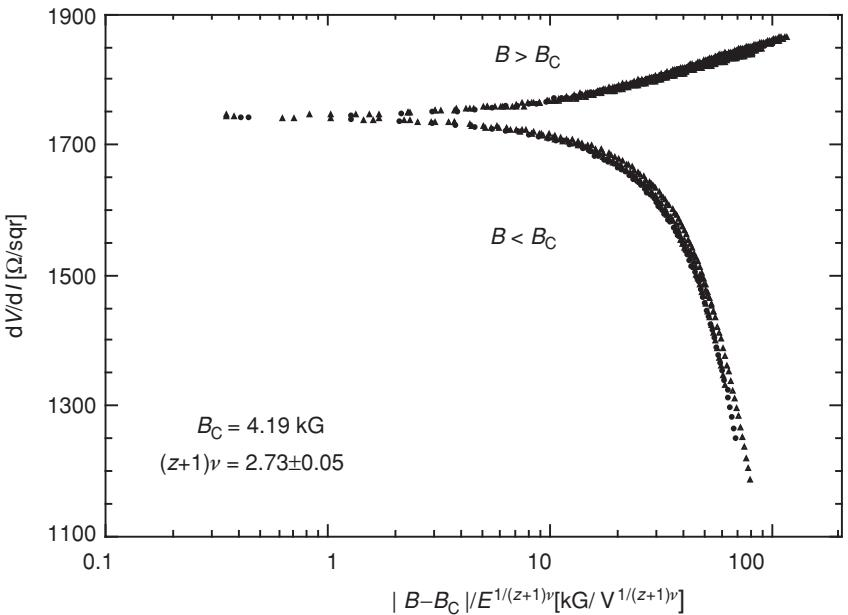
\includegraphics[width=0.6\textwidth]{figs/ch14/fig_14.2.jpg}
\caption*{图 14.2\quad MoGe 薄膜绝缘体–超导体转变中方块电阻 $(\mathrm{d}V/\mathrm{d}I)$ 随外加电场的数据坍缩。调控参量是磁场 $B$，临界值为 $B_{\mathrm{c}}=4.19\,\mathrm{kG}$。由温度标度得 $z\nu=1.36$，而 $(z+1)\nu=2.73$ 使电场依赖关系坍缩。数据取自 A. Yazdani and A. Kapitulnik, Phys. Rev. Lett. \textbf{74}, 3037 (1995)。}\label{fig:auto:14.2}
\end{figure}

\section{平均场解}

纯相位模型的哈密顿量在相位角差上含有一个非线性项。由于这一非线性，该模型在二维下难以严格处理。然而，通过极小化配分函数中出现的自由能，我们可以得到一个具有正确定性特征的平均场解。我们不用作用量来写配分函数，而是采用一个便于微扰论的形式。配分函数

\begin{equation*}
Z = \mathrm{Tr}\,\exp\left[ -\beta(H_0+H_1) \right] = \mathrm{Tr}\left[ \rho \right],\tag{14.15}
\end{equation*}

是对整个系统密度矩阵的迹。让我们定义 $\rho_0=\exp(-\beta H_0)$ 及其相应的配分函数 $Z_0=\mathrm{Tr}\rho_0$，其中 $H_0$ 是量子转子哈密顿量的动能项。遵循费曼（F1972）的做法，我们对 $\mathrm{e}^{\beta H_0}\rho$ 求导，得到

\begin{equation*}
\frac{\partial}{\partial\beta} \left( \mathrm{e}^{\beta H_0}\rho \right) = -\mathrm{e}^{H_0\beta} H_1\rho.\tag{14.16}
\end{equation*}

该方程的形式解为

\begin{equation*}
\rho = \rho_0 T \exp\left[ -\int_0^{\beta} \mathrm{d}\tau\, \hat{H}_1(\tau) \right],\tag{14.17}
\end{equation*}

其中 $T$ 表示编时乘积。于是，配分函数被变换为

\begin{equation*}
Z = Z_0 \left. T \exp\left( -\int_0^{\beta} \mathrm{d}\tau\, \hat{H}_1(\tau) \right) \right.,\tag{14.18}
\end{equation*}

其中 $\langle\cdots\rangle\equiv\langle\rho_0\cdots\rangle/Z_0$，而 $\hat{H}_1(\tau)$ 是算符 $H_1$ 的相互作用绘景。配分函数现在处于可以对相互作用作幂级数微扰展开的形式。我们此处的推导将紧密沿用 Doniach（D1981）的原始处理。为此，我们定义二分量矢量 $\mathbf{S}_i=(\cos\theta_i,\sin\theta_i)$ 及其傅里叶分量

\begin{equation*}
\mathbf{S}_{\mathbf{k}} = \frac{1}{\sqrt{N}} \sum_i \mathbf{S}_i\, \mathrm{e}^{\mathrm{i}\mathbf{k}\cdot\mathbf{R}_i}.\tag{14.19}
\end{equation*}

我们的配分函数工作形式即为

\begin{equation*}
Z = Z_0 \left. T \exp\left( \int_0^{\beta} \mathrm{d}\tau \sum_{\mathbf{k}} J_{\mathbf{k}} \mathbf{S}_{\mathbf{k}}(\tau)\cdot\mathbf{S}_{\mathbf{k}}^{*}(\tau) \right) \right.,\tag{14.20}
\end{equation*}

其中

\begin{equation*}
J_{\mathbf{k}} = \frac{J}{N} \sum_{\langle ij\rangle} \mathrm{e}^{\mathrm{i}\mathbf{k}\cdot\mathbf{R}_{ij}} = J_0(\cos k_x + \cos k_y),\tag{14.21}
\end{equation*}

$J_0=J\alpha$，$\alpha$ 是近邻的数目。

还需要一个中间步骤。用离散的松原（Matsubara）频率 $\omega_l=2\pi l T,\ l=0,\pm 1,\pm 2,\ldots$，我们把自旋矢量改写为

\begin{equation*}
\mathbf{S}_{\mathbf{k}}(\tau) = \frac{1}{\sqrt{\beta}} \sum_l \mathrm{e}^{\mathrm{i}\omega_l\tau} \mathbf{S}_{\mathbf{k}\omega_l}, \quad 0\le\tau\le\beta,\tag{14.22}
\end{equation*}

它们在虚时间区间 $0\le\tau\le\beta$ 上归一化。这使我们能把配分函数中出现的指数

\begin{equation*}
\exp\left[ \int_0^{\beta} \mathrm{d}\tau \sum_{\mathbf{k}} J_{\mathbf{k}} \mathbf{S}_{\mathbf{k}}(\tau)\cdot\mathbf{S}_{\mathbf{k}}^{*}(\tau) \right] = \prod_{\mathbf{k},l} \exp\left[ J_{\mathbf{k}} |\mathbf{S}_{\mathbf{k},l}|^2 \right],\tag{14.23}
\end{equation*}

简化成一个乘积。我们用哈伯德–斯特拉托诺维奇（Hubbard--Stratonovich）变换的复数形式（H1959；S1958）来解耦式 (14.23) 中的二次自旋相互作用

\begin{equation*}
\mathrm{e}^{-\lambda|a|^2} = \int\!\!\int \frac{\mathrm{d}(\mathrm{Re}\,\psi)(\mathrm{Im}\,\psi)}{\pi}\, \mathrm{e}^{-\left[ |\psi|^2 + \sqrt{\lambda}(a\psi^*+a^*\psi) \right]},\tag{14.24}
\end{equation*}

这是多体物理中常用的技巧，用于简化配分函数中出现的相互作用项。这一变换带来一个对辅助场的额外积分，它通常可以用最陡下降法完成。在式 (14.20) 中使用这一变换后，我们得到简化后的配分函数

\begin{equation*}
Z = \frac{Z_0}{D} \int \prod \mathcal{D}\psi_{\mathbf{k}}(\tau)\, \mathrm{e}^{-\mathcal{F}[\psi]},\tag{14.25}
\end{equation*}

其中 $\mathcal{F}$ 是自由能

\begin{align*}
\mathcal{F}[\psi_{\mathbf{k}}(\tau)] &= \sum_{\mathbf{k}} \int_0^{\beta} \mathrm{d}\tau\, \frac{\psi_{\mathbf{k}}^{*}(\tau)\cdot\psi_{\mathbf{k}}(\tau)}{J_{\mathbf{k}}} \\
&\quad -\ln\left[ \left. T \exp\left[ -2\int_0^{\beta} \mathrm{d}\tau \sum_{\mathbf{k}} \psi_{\mathbf{k}}(\tau)\cdot\mathbf{S}_{-\mathbf{k}}(\tau) \right] \right. \right],\tag{14.26}
\end{align*}

以及 $D=\pi\prod_{\mathbf{k}}J_{\mathbf{k}}$。在得到自由能的这一形式时，我们对辅助场作了重新标度 $\psi_{\mathbf{k}}\rightarrow\psi_{\mathbf{k}}/\sqrt{J_{\mathbf{k}}}$。

在平均场近似中，我们假设 $\psi$ 为常数。此外，我们可以自由选择 $\psi$ 的取向。为方便起见，我们让 $\psi$ 沿 $x$ 轴取向，于是 $\psi_{\mathbf{k}}=\sqrt{N}\delta_{\mathbf{k},0}\psi_x$。把这个辅助场形式代入式 (14.26)，得到自由能的平均场表达式

\begin{equation*}
\mathcal{F}[\psi_{\mathbf{k}}]_{\mathrm{MF}} = \frac{\beta N \psi_x^2}{J_0} - \ln\left[ \left. T \exp\left[ -2\int_0^{\beta} \psi_x \sum_i S_i^x(\tau)\,\mathrm{d}\tau \right] \right. \right]\tag{14.27}
\end{equation*}

假设 $\psi$ 是一个小参量，我们就可以自由地展开指数：

\begin{align*}
& \left. T \exp\left[ -2\int_0^{\beta} \psi_x \sum_i S_i^x(\tau)\,\mathrm{d}\tau \right] \right. = 1 - 2\psi_x \left. \int_0^{\beta} \sum_i S_i^x(\tau)\,\mathrm{d}\tau \right. \\
& \quad + 2\psi_x^2 \left. T \int_0^{\beta}\int_0^{\beta} \mathrm{d}\tau\,\mathrm{d}\tau' \sum_{ij} S_i^x(\tau) S_j^x(\tau') \right. + \cdots.\tag{14.28}
\end{align*}

物理上，这个展开中的各项代表序参量的相位涨落。如果这些项导致自由能变号，相变就会发生。为了计算这些平均值，我们在自由转子本征态

\begin{equation*}
\langle m|\theta\rangle = \frac{1}{2\pi}\,\mathrm{e}^{\mathrm{i}m\theta}.\tag{14.29}
\end{equation*}

中展开。在这个基下

\begin{equation*}
H_0\langle m_i|\theta_i\rangle = m_i^2 E_{\mathrm{C}} \langle m_i|\theta_i\rangle,\tag{14.30}
\end{equation*}

这立即给出零阶配分函数的紧凑形式

\begin{equation*}
Z_0 = \mathrm{Tr}\,\mathrm{e}^{-\beta H_0} = \sum_{\{m_i\}} \mathrm{e}^{-\beta E_{\mathrm{C}} \sum_i m_i^2}\tag{14.31}
\end{equation*}

这一基选法的另一个后果是，线性于 $S_i^x$ 的平均值恒为零

\begin{equation*}
\langle m_i|\cos\theta_i|m_i\rangle = \int_0^{2\pi} \frac{\mathrm{d}\theta_i}{2\pi}\, \mathrm{e}^{-\mathrm{i}m_i\theta_i}\, \cos\theta_i\, \mathrm{e}^{\mathrm{i}m_i\theta_i} = 0.\tag{14.32}
\end{equation*}

因此，精确到 $\psi$ 的最低阶，式 (14.28) 中二阶项只有对角元（$i=j$）给出非零结果。把式 (14.28) 代入式 (14.27) 并对 $\psi$ 求导，我们得到最低阶的鞍点方程

\begin{align*}
\frac{\beta}{J_0} &= 2\left. T \int_0^{\beta}\int_0^{\beta} \mathrm{d}\tau\,\mathrm{d}\tau'\, S_i^x(\tau) S_i^x(\tau') \right. \\
&= 2\int_0^{\beta} \mathrm{d}\tau\,\mathrm{d}\tau'\, C_0(\tau-\tau')\tag{14.33}
\end{align*}

其中

\begin{equation*}
C_0(\tau-\tau') = \frac{1}{Z_0} \sum_{\{m_i\}} \mathrm{e}^{-\beta E_{\mathrm{C}} \sum_i m_i^2}\, \langle\{m_i\}| T \hat{S}_i^x(\tau) \hat{S}_i^x(\tau') |\{m_i\}\rangle\tag{14.34}
\end{equation*}

是相位涨落关联函数。这是进入量子转子模型相变平均场理论的关键量。

$S_i^x$ 唯一的非零矩阵元具有形式

\begin{equation*}
\langle m_i|\cos\theta_i|m_i\pm 1\rangle = \frac{1}{2},\tag{14.35}
\end{equation*}

于是关联函数由下式给出

\begin{equation*}
\langle\{m_i\}| T \hat{S}_i^x(\tau) \hat{S}_i^x(\tau') |\{m_i\}\rangle = \frac{1}{2}\, \mathrm{e}^{-E_{\mathrm{C}}|\tau-\tau'|}\, \cosh(2m_i E_{\mathrm{C}}(\tau-\tau'))\tag{14.36}
\end{equation*}

这个表达式有两个重要极限。在 $E_{\mathrm{C}}\beta\gg 1$ 的低温下，所有转子都可以当作处于各自的基态，即 $m_i=0$。此时关联函数约化为一个指数

\begin{equation*}
C_0(\tau-\tau') = \frac{1}{2}\, \mathrm{e}^{-E_{\mathrm{C}}|\tau-\tau'|}, \quad \beta E_{\mathrm{C}}\gg 1,\tag{14.37}
\end{equation*}

而平均场稳定性条件

\begin{equation*}
1 = \frac{2J_0}{E_{\mathrm{C}}} \left[ 1 - \frac{1-\mathrm{e}^{-\beta E_{\mathrm{C}}}}{\beta E_{\mathrm{C}}} \right], \quad \beta E_{\mathrm{C}}\gg 1\tag{14.38}
\end{equation*}

在完成式 (14.33) 中的时间积分后随即得到。准确到 $1/\beta$ 的领头阶，我们发现耦合常数 $g=E_{\mathrm{C}}/J_0$ 的稳定性条件为

\begin{equation*}
g = 2\left( 1 - \frac{T}{E_{\mathrm{C}}} \right) + O(T^2/J).\tag{14.39}
\end{equation*}

因此，$T=0$ 处耦合常数的临界值为 $g_{\mathrm{c}}=2$。对 $g>g_{\mathrm{c}}$，量子涨落占主导，系统处于相位无序区。

在高温下，必须在式 (14.33) 的时间积分中保留关联函数的完整表达式，即式 (14.36)

\begin{align*}
& \frac{1}{2}\int_0^{\beta}\mathrm{d}\tau\int_0^{\beta}\mathrm{d}\tau'\, \mathrm{e}^{-E_{\mathrm{C}}|\tau-\tau'|}\, \cosh 2m_i E_{\mathrm{C}}|\tau-\tau'| \\
& \quad = \frac{1}{2}\sum_{\sigma} \left[ \frac{\beta}{E_{\mathrm{C}}(1+2\sigma m_i)} - \frac{1-\mathrm{e}^{-\beta E_{\mathrm{C}}(1+2\sigma m_i)}}{E_{\mathrm{C}}^2(1+2\sigma m_i)^2} \right],\tag{14.40}
\end{align*}

其中 $\sigma=\pm 1$。对 $m_i$ 求和的主要贡献来自 $m_i<1/\beta E_{\mathrm{C}}$。然而，由于 $\beta E_{\mathrm{C}}\ll 1$，我们展开式 (14.40)，只保留与 $m_i$ 无关的项。于是，式 (14.34) 中对 $m_i$ 的求和被分母中的 $Z_0$ 因子抵消，立即得到高温下的稳定性条件

\begin{equation*}
k_{\mathrm{B}}T = J_0 - \frac{E_{\mathrm{C}}}{3} + O((E_{\mathrm{C}}/J)^2)\tag{14.41}
\end{equation*}

临界温度即为 $T_{\mathrm{c}}=J_0/k_{\mathrm{B}}$。作为耦合常数 $g$ 的函数、连接高温区与低温区的平均场相边界示于图 14.3。虽然这是一张平均场相图，它却抓住了二维系统中由相位涨落导致超导电性被破坏的正确定性特征。图 14.3 中有限温度线的更精确描述应归功于别列津斯基（Berezinskii，B1971）以及科斯特利兹和索利斯（Kosterlitz and Thouless，KT1973）。别列津斯基–科斯特利兹–索利斯（Berezinskii--Kosterlitz--Thouless，BKT）相变的精髓在于：有序相以束缚的涡旋–反涡旋对为特征。临界点上涡旋的解绑导致耗散以及电阻态的出现。凭借该模型中电荷与涡旋之间的内禀对偶性（F1990），纯相位模型可以理解为涡旋–反涡旋解绑转变。这种对偶性规定：在转变的超导侧，涡旋是束缚的，而库珀对凝聚在具有刚性相位的态中；在无序侧，凝聚的是涡旋，而库珀对保持局域化。在二维荷电超流体的语境中，涡旋解绑的条件

\begin{figure}[H]\centering
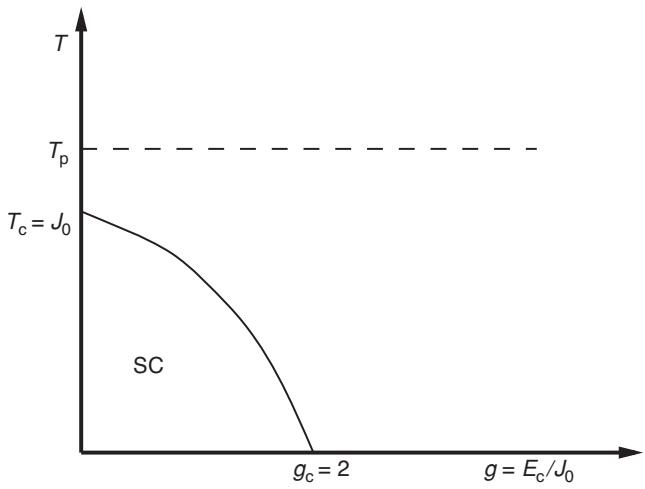
\includegraphics[width=0.5\textwidth]{figs/ch14/fig_14.3.jpg}
\caption*{图 14.3\quad 量子转子模型的平均场相图。实线表示二阶临界点的连续线。转变温度与量子临界点的平均场值分别为 $T_{\mathrm{c}}/J_0=1$ 和 $g_{\mathrm{c}}=2$。越过实线后相位相干丧失，标志着超导态不复存在。$T_{\mathrm{p}}$ 标示配对振幅开始出现的温度尺度。}\label{fig:auto:14.3}
\end{figure}

\begin{equation*}
k_{\mathrm{B}} T_{\mathrm{BKT}} = \frac{\pi\hbar^2 n_{\mathrm{s}}(T)}{2m^*},\tag{14.42}
\end{equation*}

只依赖于超流密度 $n_{\mathrm{s}}(T)$ 与载流子的有效质量 $m^*$。注意，平均场条件 $T_{\mathrm{c}}=J_0$ 与 $T_{\mathrm{BKT}}$ 相当类似，因为约瑟夫森耦合 $J_0$ 正比于超流密度。由于无序消耗超流密度，$T_{\mathrm{BKT}}$ 线应当与正常态面电阻成反比（BMO1979；HN1979）。无序超过临界值后，超流密度消失，相位有序态终止。因此，无序可以调计涡旋解绑转变。事实上，量子转子模型的系统参量可以用正常态面电阻 $R_{\mathrm{N}}$ 改写。约瑟夫森耦合 $J_0$ 正比于零温能隙、反比于无序，大致按 $R_{\mathrm{N}}^{-1}$ 标度。当无序增大时，约瑟夫森岛的尺寸减小，因而充电能增大。结果 $E_{\mathrm{C}}$ 随 $R_{\mathrm{N}}$ 增大。遵循 Simanek（S1980），我们作近似 $E_{\mathrm{C}}\propto R_{\mathrm{N}}$。于是 $g\propto R_{\mathrm{N}}^2$，当正常面电阻超过临界值时纯相位模型具有一个临界点，与实验观测一致（HP1990；J1989）。虽然把无序设想为 $R_{\mathrm{N}}$ 增大的机制最为自然，其他外部扰动（如外加磁场）也同样奏效。MoGe 薄膜中超导态被磁场调计而摧毁的过程示于图 14.2。

由于一开始就假设了配对的存在，图 14.3 中所示的 $T_{\mathrm{BKT}}$ 或平均场 $T_{\mathrm{c}}$ 必定低于配对振幅首次变为非零的温度。配对形成的温度尺度在图 14.3 中以 $T_{\mathrm{p}}$ 标示。在 $T_{\mathrm{c}}$ 和 $g_{\mathrm{c}}$ 以上，系统是相位无序的。这一点至关重要：在二维，配对形成与相位相干的能量尺度是解耦的。这种情况源于二维中相位涨落的剧烈程度。此外，在 $g_{\mathrm{c}}$ 附近，温度连续地降到零，表明相变是二阶的。一旦温度在 $g_{\mathrm{c}}$ 处升高，经典涨落便出现了。恰在 $g_{\mathrm{c}}$ 上方，动力学由温度控制。这个区域一般被称为“量子临界”区，因为系统在有序相与无序相之间被撕扯。理解这种竞争需要计算作为 $g$ 的函数的关联长度。为此，我们求助于量子转子模型的一个有效的朗道描述。

\section{朗道–金兹堡理论}

量子转子模型表述的最后一步，是把相应的自由能泛函改写成朗道理论的形式。为此，我们考虑式 (14.26) 中的自由能形式。首先，把辅助场写成对离散松原频率的求和

\begin{equation*}
\psi_{\mathbf{k}}(\tau) = \frac{1}{\sqrt{\beta}} \sum_l \mathrm{e}^{\mathrm{i}\omega_l\tau} \psi_{\mathbf{k},\omega_l},\tag{14.43}
\end{equation*}

其中傅里叶变换后的场由下式给出

\begin{equation*}
\psi_{\mathbf{k},\omega_l} = \frac{1}{\sqrt{\beta}} \int_0^{\beta} \psi_{\mathbf{k}}(\tau)\, \mathrm{e}^{-\mathrm{i}\omega_l\tau}\,\mathrm{d}\tau.\tag{14.44}
\end{equation*}

接下来，我们展开式 (14.27) 中的对数，并记住由式 (14.32)，$\psi$ 的奇次幂为零。于是，自由能

\begin{equation*}
\mathcal{F}[\psi] = \sum_{\mathbf{k},l,l'} \psi_{\mathbf{k},l}^{*} \psi_{\mathbf{k},l'} \left[ J_{\mathbf{k}}^{-1} \delta_{l,l'} - 2 C_0(\omega_l, \omega_{l'}) \right] + O(\psi^4) + \cdots\tag{14.45}
\end{equation*}

只含 $\psi$ 的偶次幂。频率依赖的自旋关联函数

\begin{align*}
C_0(\omega_l, \omega_{l'}) &= \frac{1}{\beta}\int_0^{\beta}\int_0^{\beta} \mathrm{d}\tau\,\mathrm{d}\tau'\, C_0(\tau,\tau')\, \mathrm{e}^{\mathrm{i}\omega_l\tau}\, \mathrm{e}^{-\mathrm{i}\omega_{l'}\tau} \\
&= \delta_{ll'} \frac{E_{\mathrm{C}}}{E_{\mathrm{C}}^2+\omega_l^2} \approx \delta_{ll'} \frac{1}{E_{\mathrm{C}}} \left( 1 - \frac{\omega_l^2}{E_{\mathrm{C}}^2} \right)\tag{14.46}
\end{align*}

在低温下，即 $C_0(\tau,\tau')\propto\exp{-E_{\mathrm{C}}|\tau-\tau'|}$ 时，具有简单的形式。四阶项的类似关联函数也可以算出。然而，其精确系数——我们启发式地记作 $U$——在这个语境中并不特别重要。由于我们的焦点是长波物理，我们展开 $J_{\mathbf{k}}$，只保留二次项 $J_{\mathbf{k}}\approx J_0(1-(ka)^2/2)$，其中 $a$ 是晶格常数。把这些结果与式 (14.45) 和式 (14.46) 的结果合并，我们立即看到自由能

\begin{align*}
\mathcal{F}[\psi] &= \sum_{\mathbf{k},l} \psi_{\mathbf{k},l}^{*} \psi_{\mathbf{k},l} \left[ \left( \frac{1}{J_0} - \frac{2}{E_{\mathrm{C}}} \right) + \frac{(ka)^2}{2J_0} + 2\frac{\omega_l^2}{E_{\mathrm{C}}^3} \right] \\
&\quad + \frac{U}{2\beta} \sum_{\substack{\omega_1,\cdots,\omega_4 \\ \mathbf{k}_1,\ldots,\mathbf{k}_4}} \delta_{\omega_1+\cdots+\omega_4,0}\, \delta_{\mathbf{k}_1+\cdots+\mathbf{k}_4,0}\, \psi_{\omega_1,\mathbf{k}_1}^{*} \psi_{\omega_2,\mathbf{k}_2}^{*} \psi_{\omega_3,\mathbf{k}_3} \psi_{\omega_4,\mathbf{k}_4}\tag{14.47}
\end{align*}

具有朗道–金兹堡形式。注意，零温量子临界点的平均场解是 $J_0^{-1}=2/E_{\mathrm{C}}$，等价地 $(1/J_0-2/E_{\mathrm{C}})=(g-g_{\mathrm{c}})/E_{\mathrm{C}}$，这意味着二次项的常数系数正比于逆关联长度（inverse correlation length）。这一项扮演第 12 章式 (12.14) 中 $a(T)$ 的角色。此外，频率的二次依赖源于式 (14.30) 中对 $\theta$ 的两个导数。在时域中，频率的二次依赖转化为对时间的二阶导数，如式 (14.12) 所示。于是，在实空间中，自由能密度

\begin{equation*}
\mathcal{F}[\psi] = \int \mathrm{d}^2r \int \mathrm{d}\tau \left[ |\nabla\psi(\mathbf{r},\tau)|^2 + |\partial_{\tau}\psi(\mathbf{r},\tau)|^2 + \delta|\psi(\mathbf{r},\tau)|^2 + \frac{U}{2}|\psi(\mathbf{r},\tau)|^4 \right]\tag{14.48}
\end{equation*}

在对耦合常数、松原频率以及 $\psi$ 场作适当重新标度后，取人们熟悉的朗道–金兹堡形式。我们已定义 $\delta=g-g_{\mathrm{c}}$ 并取 $\hbar=c=1$。与第 12 章早先给出的朗道–金兹堡理论表述（式 (12.14)）不同而为式 (14.48) 所有的，是对虚时间的显式积分以及正比于 $\partial_{\tau}^2$ 的量子涨落项。空间与时间之间的对称性得到保证，因为自由能中时间导数与空间导数的数目相等。于是，我们认定

\begin{equation*}
\epsilon_k = \pm\sqrt{k^2+\delta}\tag{14.49}
\end{equation*}

为单粒子谱的色散关系。在超导相中 $\delta=0$，我们恢复对动量呈线性的色散关系，正如玻色子所预期的那样。然而，当量子涨落占主导时色散关系有能隙，$\delta>0$。临界点划分了有能隙（$g>g_{\mathrm{c}}$）与自由（$g<g_{\mathrm{c}}$）准粒子激发之间的转变。在相变两侧，库珀对都完好无损。因此，朗道–金兹堡理论中固有的相变不是破对型的，而是由序参量 $\psi(\omega,\mathbf{k})$ 的相位涨落驱动。

四阶项的作用是把准粒子散射纳入关联长度。定量刻画这一效应的最简单方法是使用哈特里–福克理论。在此框架下，我们可以通过对场 $\psi_{\mu}$ 的分量数目 $N$ 作展开来实现这一步骤，其中 $\mu$ 是每个分量的指标。对转子问题，$\psi_{\mu}$ 是一个二分量场。哈特里–福克步骤相当于取 $N\rightarrow\infty$ 极限。如果 $1/N$ 幂次的修正证明很小，那么一旦我们用 $U/N$ 替换 $U$，大 $N$ 展开就为处理自由能中的四次项提供了一条简便途径。我们将看到，$1/N$ 展开无法重现有限温度相变。然而，它对勾画环绕量子临界点的各个不同区域颇有启发。

为了得到关联长度，我们将自由能指数化，并使用哈伯德–斯特拉托诺维奇（H1959；S1958）变换的一个略微修改的形式

\begin{align*}
& \exp\left\{ \frac{UT}{2N} {\sum_{\substack{\omega_1,\cdots,\omega_4 \\ \mathbf{k}_1,\cdots,\mathbf{k}_4}}}^{\prime} \psi_{\mu}^{*}(\omega_1,\mathbf{k}_1) \psi_{\mu}^{*}(\omega_2,\mathbf{k}_2) \psi_{\nu}(\omega_3,\mathbf{k}_3) \psi_{\nu}(\omega_4,\mathbf{k}_4) \right\} \\
&\quad = \int \mathcal{D}\lambda \exp\left\{ -\frac{N}{2U} \sum_{\mathbf{k}} |\lambda(\omega,\mathbf{k})|^2 \right. \\
&\qquad \left. + \frac{1}{\sqrt{\beta}} \sum_{\mathbf{k}_1,\mathbf{k}_2,\omega_1,\omega_2} \lambda(\omega_1-\omega_2, \mathbf{k}_1-\mathbf{k}_2) \psi_{\mu}(\omega_1,\mathbf{k}_1) \psi_{\mu}(-\omega_2,-\mathbf{k}_2) + \mathrm{hc} \right\},\tag{14.50}
\end{align*}

来解耦四次项，其中撇号表示约束 $\delta_{\omega_1+\cdots+\omega_4,0}$ 与 $\delta_{\mathbf{k}_1+\cdots+\mathbf{k}_4,0}$。在鞍点近似中，辅助场是一个常数：$\lambda(\omega,k)=\sqrt{\beta}\lambda\delta_{\omega,0}\delta_{\mathbf{k},0}$。把这个表达式代入配分函数并对 $\lambda$ 极小化，得到大 $N$ 极限下 $\lambda$ 的鞍点方程

\begin{equation*}
\lambda = \frac{U}{\beta} \sum_{\omega_m} \int \frac{\mathrm{d}^2k}{(2\pi)^2}\, \frac{1}{\delta+k^2+\omega^2+\lambda}\tag{14.51}
\end{equation*}

令 $m^2=\delta+\lambda$ 为逆关联长度的平方。临界点现在由 $m=0$ 确定。一旦在式 (14.51) 中完成对动量的积分，就可以用泊松求和技术（见习题 14.4）计算对松原频率的求和。由此得到的自洽条件

\begin{equation*}
m^2 = \delta + \frac{UT}{2\pi} \ln\left( \frac{\sinh\sqrt{\Lambda^2+m^2}/2T}{\sinh m/2T} \right)\tag{14.52}
\end{equation*}

\begin{figure}[H]\centering
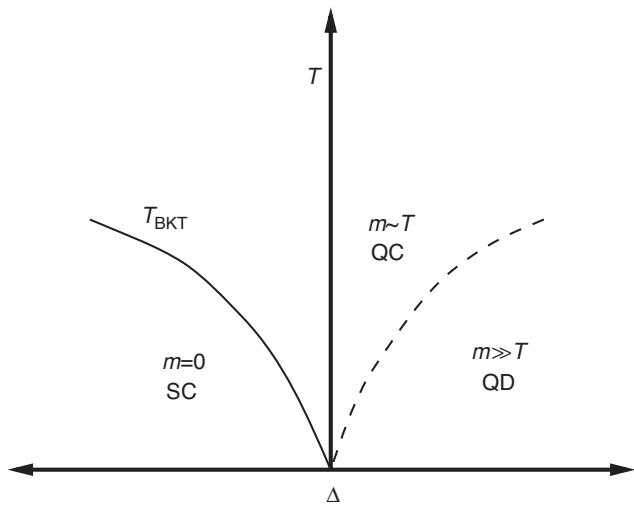
\includegraphics[width=0.5\textwidth]{figs/ch14/fig_14.4.jpg}
\caption*{图 14.4\quad 量子转子模型的有限温度相图，以温度以及到量子临界点（$\Delta=g-g_{\mathrm{c}}=0$）的距离为变量。实线 $T_{\mathrm{BKT}}$ 表示由别列津斯基–索利斯–科斯特利兹（Berezinskii--Thouless--Kosterlitz）确定的二阶临界点线。实线以下，逆关联长度 $m$ 消失，相位相干得以建立。虚线表示从量子临界（QC）区——其中动力学由温度决定，$m\propto T$——到相位无序（QD）区——其中量子涨落主导，$m\gg T$——的交叉过渡（crossover）。逆关联长度在各区中的行为由式 (14.53) 给出。}\label{fig:auto:14.4}
\end{figure}

在 $T=0$ 且重正化调控参量 $\Delta=\delta+U\Lambda/4\pi$ 为零时有解 $m=0$。这里 $\Lambda$ 是动量截断。因此，平均场理论未能恢复逆关联长度消失的正确有限温度相变（BKT 型）。尽管如此，作为温度的函数，出现三个不同的区域

\begin{equation*}
m = \left\{ \begin{array}{lll}
T \exp\left\{ -\dfrac{2\pi|\Delta|}{UT} \right\}, & \Delta<0, & \text{有序相}, \\[2ex]
2\ln\dfrac{\sqrt{5}+1}{2}\, T, & |\Delta|\ll T, & \text{量子临界}, \\[2ex]
\dfrac{4\pi\Delta}{U}, & \Delta>0, & \text{量子无序},
\end{array} \right.\tag{14.53}
\end{equation*}

它们刻画所有量子相变。展示这些区域的相图示于图 14.4。有序相出现在临界点 $\Delta=0$ 的左侧（$\Delta<0$），其特征是在某个温度以下逆关联长度消失。图 14.4 中的实线表示二阶临界点的 $T_{\mathrm{BKT}}$ 线。对 $N=2$，有序态是超导体。$N=1$ 的有序态对应铁磁体，因而属于二维伊辛模型的普适类。对 $N\ge 3$，有限温度相变线被压低到 $T=0$，从而表明不存在有限温度有序态。由式 (14.53) 可以立刻看出 $1/N$ 展开无法给出有限温度相变，因为对 $\Delta<0$，$m$ 仅在 $T=0$ 时才消失。在 $\Delta=0$ 的正上方，系统交叉过渡到一个中间区域，在其中热涨落而非量子涨落决定动力学。在此区域中，逆关联长度随温度线性变化，且其系数是普适的。该区域被称为量子临界区，因为系统正试图判定两个基态中哪一个更可取。处于这种不定态的一切体系的一个基本特征是：所有能标——或等价地，所有弛豫速率——随温度线性标度。因此，正如引言中所讨论的，在量子临界区，准粒子激发并非良定义的。随着 $\Delta$ 增大，系统从量子临界区交叉过渡到量子无序区。在这一极限下，温度退居次要地位，序参量的量子涨落决定物理。于是 $\langle\psi^{*}(\mathbf{r})\psi(\mathbf{r})\rangle\propto\exp(-r/\xi)\propto\exp(-mr)$。此区域中的能量激发是有能隙的，由 $\epsilon_{k}=\sqrt{k^{2}+m^{2}}$ 给出。

\section{输运性质}

电导率既是频率的函数，也是温度的函数。到临界点的距离同样决定着电导率。于是有 $\sigma=\Sigma(\hbar\omega,T,\Delta)$。考虑 $\Delta=0$ 的简单情形。零温输运性质应当如何确定？由于量子临界点出现在 $T=0$，合理的假设似乎是：正确的 $T=0$ 极限由 $\Sigma(\hbar\omega,T=0,0)$ 得到，而直流电导率则通过取零频极限获得。这当然假定了频率依赖与温度依赖是解耦的。若二者确实解耦，则 $\omega\to0,\,T=0$ 与 $\omega=0,\,T\to0$ 这两个极限便可交换次序。

Damle 与 Sachdev 在一篇开创性的论文 [DS1997] 中证明，在量子临界点附近，这两个极限毕竟不可交换。他们的论证基于如下观察：在量子临界点附近，电导率是 $\hbar\omega/k_{\mathrm{B}}T$ 的普适函数。这意味着 $\Sigma(\hbar\omega/k_{\mathrm{B}}T)$ 存在两个截然不同的 $T\to0$ 极限：一个极限是 $\Sigma(\hbar\omega\to0,T=0)=\Sigma(\infty)$，另一个是 $\Sigma(\omega=0,T\to0)=\Sigma(0)$。Damle 与 Sachdev 的要点在于 $\Sigma$ 是单调函数，因而 $\Sigma(0)\neq\Sigma(\infty)$。实验上，直流输运性质的一切测量都是在 $\hbar\omega\ll k_{\mathrm{B}}T$ 的极限下进行的，因此与实验相关的是 $\Sigma(0)$ 这一极限。早期关于绝缘体–超导体转变的全部理论工作 [C1991; WZ1990; KZ1993; W1994] 都基于极限形式 $\Sigma(\infty)$。该极限对应于相干区域，即高频极限，其中由外加电场引起的弛豫决定输运性质。然而相反的区域在性质上截然不同。在极限形式 $\Sigma(0)$ 中，热激发准粒子之间的碰撞支配一切弛豫过程。为描述这一区域，必须针对准粒子散射建立一个量子动理学方程（quantum kinetic equation），它与为金属中声子主导的输运所建立的玻尔兹曼方法直接类似。这里的关键意外在于：若不分析有限温弛豫过程，便无法理解 $T=0$ 量子临界点的输运性质。

为说明频率与温度趋于零这两个极限的不可交换性会如何剧烈地影响电导率，考虑量子无序区。在此区域中 $m\gg T$，能隙之上存在热激发的准粒子。然而，按朴素的考虑，能隙的存在意味着直流电导率应当为零。但事实并非如此。量子无序区中 $m\gg T$ 的约束意味着相关动量满足 $k<\sqrt{mT}<m$。于是色散关系可以写成
\begin{equation*}
\epsilon_{\mathbf{k}}\approx m+\frac{k^{2}}{2m}\approx m,\quad m\gg T,\tag{14.54}
\end{equation*}
而准粒子统计在量子无序区成为玻尔兹曼型的。因此，准粒子的布居指数地小。然而，准粒子布居的这种指数式稀少同时也导致指数式小的散射概率。精确计算 [DP2001] 表明，在量子无序区，散射率
\begin{equation*}
\frac{1}{\tau}=\pi T\,\mathrm{e}^{-m/T}\tag{14.55}
\end{equation*}
与动量无关，并由同一个压制准粒子布居的指数因子支配。由爱因斯坦关系，电导率是准粒子密度与散射时间的乘积。两个指数因子相互抵消 [DP2001]，给出电导率
\begin{equation*}
\sigma_{\mathrm{qd}}=\frac{2}{\pi}\,\frac{4e^{2}}{h}\tag{14.56}
\end{equation*}
它在 $m\ll1$ 时有限。在离临界点更远处，该系数会被相互作用的具体形式修正。尽管如此，直流电导率仍然保持有限。此外，散射率中的所有对数贡献 [DP2001] 在低温下都消失，因而不影响 $T=0$ 处有限的直流电导率。这一论证的关键在于：一旦准粒子服从玻尔兹曼统计，散射事件便变得稀少。因此，准粒子可以在不发生散射的情况下游弋相当长的距离。于是，纯相位模型（phase-only model）的普遍相图（图 14.5）包含一个作为超导体的有序相，以及一个“金属的”相位无序区。这个“绝缘体”是一个具有有限直流电导率的金属。这是频率与温度趋于零极限的不可交换性所引出的关键意外之一。Green 与 Sondhi [GS2005] 也利用上面讨论的相消论证证明，有能隙的即量子无序的相实际上是金属性的。我们把这个相称为玻色金属（Bose metal），因为其基本激发是玻色子。在有限频率下，$\Sigma(\omega,T)$ 在 $\omega=0$ 处呈现一个洛伦兹型峰，其宽度为 $1/\tau$ 的量级。因此，实验观测玻色金属所受的约束是 $\omega\ll1/\tau$。温度为 0.1 K 时，弛豫时间为 $10^{10}\exp(-m/T)\ \mathrm{s}^{-1}$，其中 $m\gg T$。测量直流电导率时的典型实验频率为 2--27 Hz 的量级。因此，只要 $T>0.05m$，玻色金属便可以被观测到。典型情况下 $T>0.1m$。由此可见，似乎不存在任何关于频率的实验约束会妨碍对玻色金属相的观测。然而，这里描述的玻色金属是脆弱的，因为所有其他散射机制（例如无序）都会破坏导致式 (14.56) 的完美相消。因此，绝缘体–超导体转变尚待解决的问题之一，便是低温下居间金属相的起源。

\begin{figure}[H]\centering
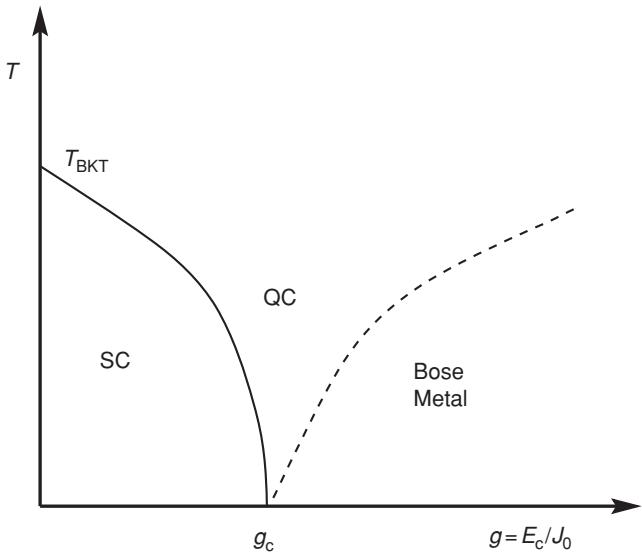
\includegraphics[width=0.6\textwidth]{figs/ch14/fig_14.5.jpg}
\caption*{图 14.5\quad 约瑟夫森结阵列中相位相干性被破坏的相图。对该体系，$g$ 由充电能量 $E_{\mathrm{C}}$ 与约瑟夫森耦合 $J_{0}$ 之比给出。$T_{\mathrm{BKT}}$ 是 Berezinskii–Kosterlitz–Thouless（BKT）温度，低于该温度时相位相干性得以建立；$g_{\mathrm{c}}$ 则给出为破坏超导相所需的相位无序的临界值。QC 指量子临界区，其中逆关联长度随温度线性变化。一旦相位相干性被破坏，便出现金属态。该金属态完全源于电导率的频率趋于零极限与温度趋于零极限之间缺乏可交换性。}\label{fig:auto:14.5}
\end{figure}

\section{实验}

纯相位模型对薄膜中绝缘体–超导体转变（insulator-superconductor transition，IST）的适用性，取决于在转变两侧都存在库珀对这一前提。因此，直接测量单粒子谱的隧穿实验是检验纯相位模型关键预言的理想手段。在颗粒薄膜上进行的这类实验 [B1994] 揭示：在转变的绝缘一侧，单粒子能隙保持有限，且相对体超导值并无衰减。因此，纯相位模型对颗粒薄膜中实验观测到的 IST 给出了准确的描述。

\begin{figure}[H]\centering
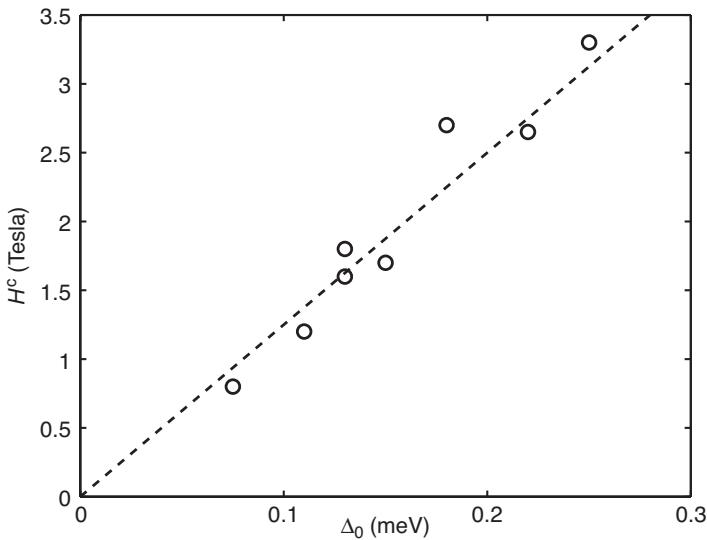
\includegraphics[width=0.55\textwidth]{figs/ch14/fig_14.6.jpg}
\caption*{图 14.6\quad PbBi/Ge 薄膜的临界磁场 $H_{\mathrm{c}}$ 对能隙 $\Delta_{0}$ 的关系图。根据 S.-Y. Hsu 的学位论文 [H1995] 重绘。}\label{fig:auto:14.6}
\end{figure}

那么，均匀无序的薄膜情形又如何呢？这里的情况颇为不同。图 14.6 给出了 PbBi/Ge 中破坏超导态所需的临界磁场随单粒子能隙的变化。显而易见，$H_{\mathrm{c}}$ 随能隙线性标度。只要 $H_{\mathrm{c}}$ 对应于库珀对破坏场 $H_{\mathrm{c2}}$，这一对应关系便在 BCS 理论的预期之内（见式 (12.207)）。事实上，Valles 及其合作者 [HCV1995] 已确定：在 $H_{\mathrm{c}}$ 处，费米能处的态密度为其正常态值的 80\%，这正是 $H_{\mathrm{c}}\approx H_{\mathrm{c2}}$ 时应有的情形。因此，样品中有相当大的一部分不含库珀对。这一观察也与 Dynes 及其合作者的一系列实验 [V1992] 相符：在这些实验中，能隙被观测到在名义临界场 $H_{\mathrm{c}}$ 处消失。对 MoGe，Yazdani 与 Kapitulnik [YK1995] 也发现 $H_{\mathrm{c}}\approx H_{\mathrm{c2}}$。总体而言，这些观察意味着：在均匀无序薄膜中，由库珀对破坏产生的类电子准粒子布居于转变的绝缘一侧。因此，要描述这些体系，必须有超越纯相位模型的物理。

这一状况其实也可以从如下实验事实推断出来：在大批均匀无序薄膜中，临界点处的电阻率 $R_{\mathrm{c}}$ 等于正常态电阻率 $R_{\mathrm{N}}$。图 14.7 给出了 Bi [GM1998] 与 MoGe [YK1995] 样品 $R_{\mathrm{c}}$ 对 $R_{\mathrm{N}}$ 的典型曲线图。正常态电阻 $R_{\mathrm{N}}$ 是 [YK1995; GM1998] 由 $T>T_{\mathrm{p}}$ 的输运测量提取的（见图 14.3）。因此，在这一温区内大量存在的只有类电子激发。临界电阻 $R_{\mathrm{c}}$ 则在远低于 $T_{\mathrm{p}}$ 的温度下提取，它表示 $R(T)$ 随调控参量的曲线族在 $T\to0$ 时单一交叉点处的电阻率。在 Bi 与 MoGe 两种薄膜中，磁场诱发 IST。从 Bi 与 MoGe 两者的数据显而易见，$R_{\mathrm{c}}\approx R_{\mathrm{N}}$。除非在 $R_{\mathrm{c}}$ 处发生了向正常基态的转变，否则这种 $R_{\mathrm{c}}\approx R_{\mathrm{N}}$ 的对应没有理由出现。由于 $R_{\mathrm{N}}$ 关联于不存在库珀对的高温物理，$R_{\mathrm{c}}\approx R_{\mathrm{N}}$ 这一事实意味着：在这些均匀无序薄膜中，绝缘态必定含有类电子准粒子。此外，在所有情形中 $R_{\mathrm{c}}$ 都略高于 $R_{\mathrm{N}}$，介于 $900\,\Omega$ 与 $8000\,\Omega$ 之间。这些数值与纯相位模型所预言的玻色子电阻量子 $h/4e^{2}=6500\,\Omega$ 显然相差悬殊，进一步表明起作用的是超越纯相位模型的物理。

\begin{figure}[H]\centering
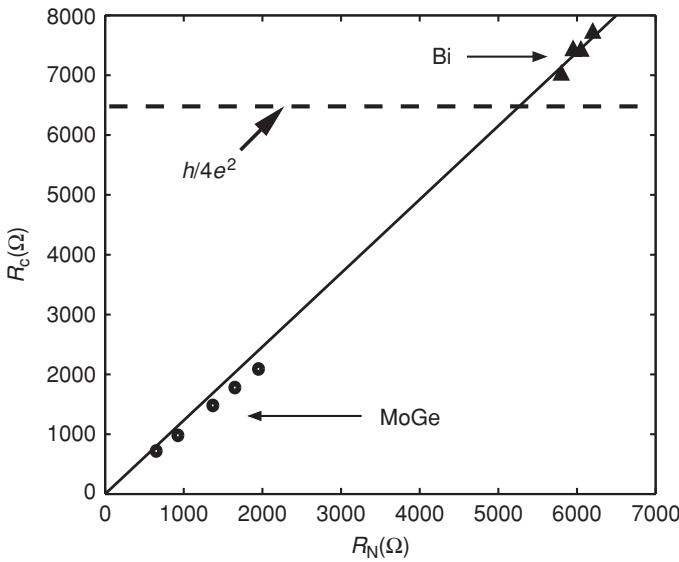
\includegraphics[width=0.55\textwidth]{figs/ch14/fig_14.7.jpg}
\caption*{图 14.7\quad Bi [GM1998] 与 MoGe [YK1995] 样品的临界电阻 $R_{\mathrm{c}}$ 随正常态电阻 $R_{\mathrm{N}}$ 的变化。转变处不存在普适值以及 $R_{\mathrm{c}}$ 与 $R_{\mathrm{N}}$ 之间的相关性表明：向绝缘态的转变中含有类电子准粒子，这正是高温正常态的特征。}\label{fig:auto:14.7}
\end{figure}

总而言之，纯相位物理似乎足以描述颗粒薄膜。然而，对大多数均匀无序薄膜，实验指向一个由类电子准粒子布居的绝缘态。因此，对破坏（pair-breaking）似乎是驱动 IST 的主导机制。由此，3d XY 模型便不再足以描述均匀无序薄膜中的 IST，因为绝缘体中存在无能隙的电子激发。在这种情形下，临界电阻便不必由 $2e$ 玻色子的电阻量子 $R_{\mathrm{Q}}=h/4e^{2}$ 界定，正如实验所观测的那样。把正常电子纳入 IST 的进展，可沿着 Feigelman 与 Larkin [FL1998] 新近采取的路线取得。

\section{标度与T线性电阻率}

量子相变受 $T=0$ 量子临界点支配。此外，由于温度起着关键作用，量子相变相应的场论是 $(d+z)$ 维的。量子转子模型是刻画超导体–非超导体量子临界点附近相互竞争的基态之间本质张力的最简单模型。该模型可以改写为金兹堡–朗道理论。$T=0$ 量子临界点的一个关键意外之处在于：输运性质必须由热激发准粒子之间的碰撞来决定。就量子转子模型而言，把准粒子散射纳入进来，会在量子无序区导致一个金属相。只要无序不是对破坏型的，玻色金属相对弱无序就是稳定的。

\begin{figure}[H]\centering
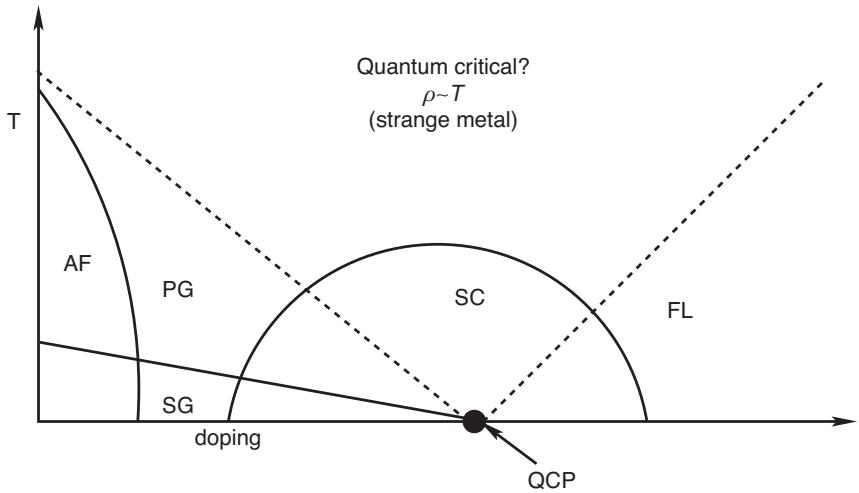
\includegraphics[width=0.72\textwidth]{figs/ch14/fig_14.8.jpg}
\caption*{图 14.8\quad 高温铜氧化物超导体的示意相图，以温度和空穴浓度（掺杂）为变量。各相为：AF 表示反铁磁体，SG 表示自旋玻璃，SC 表示具有 $d_{x^{2}-y^{2}}$ 对称性的超导体。自旋玻璃相终止于穹顶内部的一个临界掺杂水平（量子临界点，QCP）。虚线表示交叉过渡而非临界行为。在此图中，PG 与 FL 分别表示赝能隙相与费米液体相：前者的单粒子谱发展出一个凹陷，后者的输运性质变得更为常规。漏斗形区域中的奇异金属行为——$T$ 线性电阻率——曾被归因于量子临界行为。然而，对量子临界点处电导率的标度分析排除了这一情形。}\label{fig:auto:14.8}
\end{figure}

在量子临界点正上方，动力学由温度决定。因此，人们很自然地倾向于把随温度线性的电阻率与量子临界点可能的存在联系起来，铜氧化物超导体（cuprate）即属此列 [BTKW1993]。铜氧化物中的 $T$ 线性电阻率至今仍是正常态物理中的关键挑战。在铜氧化物理论的早期，人们曾引入基于某种量子临界性的解释 [T1999; V1989] 来说明 $T$ 线性电阻率。可以问一个简单的问题：量子临界性是否对由此得到的电阻率的形式施加任何限制？确实施加，这从下面的标度分析即可看出。

这一论证 [PC2005] 基于三条一般性假设：(1) 临界自由度携带电流；(2) 临界点附近只有一个长度标度是相关的；(3) 电荷守恒。倘若属实，这些假设便排除将量子临界性作为 $T$ 线性电阻率成因的可能。

考虑一个一般的作用量 $S$，只要电流是临界的，其微观细节并不重要。外加电磁矢势 $A^{\mu}$（$\mu=0,1,\ldots,d$）与电流 $j_{\mu}$ 耦合，使得
\begin{equation*}
S\to S+\int \mathrm{d}\tau\, d^{d}x\, A^{\mu}j_{\mu}.\tag{14.57}
\end{equation*}
这里的关键是矢势与电流线性耦合，因而其标度维数为 1。这一事实在后面的证明中至关重要。在量子体系的一参数标度假设下，在小于关联体积 $\xi^{d}$ 的体积内的空间关联、以及在短于 $\xi_{t}\propto\xi^{z}$ 的时间标度上的时间关联都很小，尺度为 $\xi^{d}\xi_{t}$ 的时空区域表现为独立的块体。利用这一假设，通过清点整个体系中关联体积的数目，我们写出配分函数对数之奇异部分的标度形式：
\begin{equation*}
\ln Z=\frac{L^{d}\beta}{\xi^{d}\xi_{t}}\,F\bigl(\delta\xi^{d_{\delta}},\{A_{\lambda}^{i}\xi^{d_{A}}\}\bigr).\tag{14.58}
\end{equation*}

在此表达式中，$L$ 是系统尺寸，$\delta$ 是到临界点的距离，$d_{\delta}$ 与 $d_{A}$ 分别是临界耦合与矢势的标度维数。变量 $A_{\lambda}^{i}=A^{i}(\omega=\lambda\xi_{t}^{-1})$ 对应于标度频率 $\lambda=\omega\xi_{t}$ 处的（均匀、$k=0$）电磁矢势，而 $i=1,\ldots,d$ 标记空间分量。把配分函数的对数对电磁规范场 $A^{i}(\omega)$ 取两次导数，
\begin{align*}
\sigma_{ij}(\omega,T)&=\frac{1}{L^{d}\beta}\ \frac{1}{\omega}\ \frac{\delta^{2}\ln Z}{\delta A^{i}(-\omega)\delta A^{j}(\omega)}\\
&=\xi^{-d}\ \frac{\xi_{t}^{-1}}{\omega}\ \xi^{2d_{A}}\ \frac{\delta^{2}}{\delta A_{-\bar{\lambda}}^{i}\delta A_{\bar{\lambda}}^{j}}\,F(\delta=0)\,\Big|_{\substack{\bar{\lambda}=\omega\xi_{t}\\ \{A_{\bar{\lambda}}^{i}=0\}}}\\
&=\frac{Q^{2}}{\hbar}\ \xi^{2d_{A}-d}\ \Sigma_{ij}(\omega\xi_{t}),\tag{14.59}
\end{align*}
便确定了电荷为 $Q$ 的载流子的电导率。我们已明确地取 $\delta=0$，因为我们关注的是量子临界区。在有限温度下，时间关联长度被温度截断为 $\xi_{t}\propto1/T$，且 $\xi_{t}\propto\xi^{z}$。如前所述，电磁规范场的工程量纲为 1（$d_{A}=1$）。这一结果完全源于电荷守恒 [W1992]。于是我们得到电导率的一般标度形式
\begin{equation*}
\sigma(\omega,T)=\frac{Q^{2}}{\hbar}\ T^{(d-2)/z}\ \Sigma\left(\frac{\hbar\omega}{k_{\mathrm{B}}T}\right)\tag{14.60}
\end{equation*}
其中 $\Sigma$ 只是比值 $\omega/T$ 的显函数。（为简单起见，$ij$ 张量指标已略去。）这一标度形式把 Wen [W1992] 导出的 $T=0$ 频率依赖的临界电导率推广到非零温度。这一般性标度形式，即式 (14.60)，也与 Damle 和 Sachdev [DS1997] 在其对量子临界点附近碰撞主导输运的详尽研究中所提出的形式一致（另见文献 [SS2000] 中的标度分析）。当前推导所清楚阐明的是：无论哈密顿量的底层统计或微观细节如何——无论它是玻色型的（如 Damle 与 Sachdev 的工作 [DS1997]）还是其他类型，无论有无无序——电导率的一般标度形式都保持不变。$d=2+\epsilon$ 维安德森金属–绝缘体转变（可视为以无量纲无序强度为调控参量的量子相变 [W1979; AALR1979]）的电导率（见式 (13.25)）服从这里导出的电导率标度函数。

在零频率即直流极限下，我们得到
\begin{equation*}
\sigma(\omega=0)=\frac{Q^{2}}{\hbar}\ \Sigma(0)\ \left(\frac{k_{\mathrm{B}}T}{\hbar c}\right)^{(d-2)/z}.\tag{14.61}
\end{equation*}
一般地 $\Sigma(0)\neq0$。否则，电导率将完全由自由能的非奇异、因而非临界的部分决定。铜氧化物是各向异性的三维体系。因此，对临界模式而言，相应的维数是 $d=3$ 而非 $d=2$。在后一种情形，温度前置因子是常数。对 $d=3$，我们发现仅当 $z=-1$ 时才得到 $T$ 线性电阻率。在标准的可交换（commutative）场论中，这样一个负的 $z$ 值是非物理的，因为它意味着在临界点处长波涨落的能标发散。

虽然假定 $\Sigma(0)$ 在零温下有限肯定合理，但 $\Sigma(0)$ 实际上发散也确有可能。出现这种情形的一个可能场景是：一个危险无关算符（dangerously irrelevant operator）支配着电导率。此时 $\Sigma(0)\sim1/T^{p}$，且当 $p=(d-2)/z+1$ 时得到 $T$ 线性行为。这只可能发生在上临界维数以上。在该区域，一切临界性都是平均场型的。因此，目前尚不能排除的一种可能性是：铜氧化物中的一切临界性本质上是平均场型的，而危险无关算符控制着电导率。然而，对强关联体系而言，临界性本质上是平均场型的可能性不大。

这一证明提示，下列三种可能性之一可能是相关的：(1) 量子临界性与该问题毫无关系；(2) 电流由非临界自由度携带；或 (3) 存在新的量子临界场景，其中额外的长度标度描写物理。在涉及非临界自由度的场景中，铜氧化物正常态的费米子载流子可以与一个临界玻色模式耦合。这样的解释类似于磁性体系中的情形 [H1976]：费米子从无质量玻色型密度涨落或自旋涨落上散射，导致电阻率的一系列代数形式 [K1996; R1999]，在反铁磁与铁磁体系中分别从 $T^{4/3}$ 变化到 $T^{3/2}$。虽然无序可以改变指数 [R1999]，但 $T$ 线性电阻率只在一个受限的参数空间中出现。铜氧化物中 $T$ 线性电阻率的稳健性使这类场景不太可能。我们所倡导的场景是额外长度标度进入问题的场景。这一额外自由度来自跨越莫特能隙的动力学谱权重转移。这将在最后一章中描述。

\section*{习题}
\addcontentsline{toc}{section}{习题}

\textbf{习题 14.1}\quad 在量子转子模型
\begin{equation*}
H=E_{\mathrm{C}}\sum_{i}\left(\hat{n}_{i}-n_{0}\right)^{2}-t\sum_{\langle ij\rangle}\left(b_{i}^{\dagger}b_{j}+b_{j}^{\dagger}b_{i}\right),\tag{14.62}
\end{equation*}
中，证明当 $n_{0}$ 不是整数时，相应的作用量具有如下形式：
\begin{equation*}
S\propto\int_{0}^{\beta}\mathrm{d}\tau\,\theta\partial_{\tau}\theta-\sum_{\langle ij\rangle}V(\cos\theta_{i}-\theta_{j}).\tag{14.63}
\end{equation*}
这一版本的量子转子模型称为无公度玻色–哈伯德模型（incommensurate Bose--Hubbard model）。这对动力学指数的取值有什么后果？

\textbf{习题 14.2}\quad 利用式 (14.35)，证明式 (14.36) 的结果。

\textbf{习题 14.3}\quad 利用 $C_{0}(\tau,\tau')$ 的低温形式，即式 (14.37)，建立式 (14.46) 中最后的等式。

\textbf{习题 14.4}\quad 完成式 (14.51) 中的积分，然后用泊松求和公式导出式 (14.52)。

\section*{参考文献}
\addcontentsline{toc}{section}{参考文献}

\begin{itemize}[leftmargin=2em,itemsep=0pt,parsep=0pt,label={}]
\item [AALR1979] E. Abrahams, P. W. Anderson, D. C. Licciardello, and T. V. Ramakrishnan, \emph{Phys. Rev. Lett.} \textbf{42}, 673 (1979).
\item [AR1998] G. Aeppli and T. F. Rosenbaum, in \emph{Dynamical Properties of Unconventional Magnetic Systems}, eds. A. T. Skjeltorp and D. Sherrington (Kluwer Academic Publishers, Netherlands, 1998), p. 107.
\item [A1964] P. W. Anderson, in \emph{Lectures on the Many Body Problem}, ed. E. R. Caianiello (Academic, New York, 1964), Vol. 2, p. 127.
\item [B1994] R. P. Barber, Jr., L. M. Merchant, A. La Porta, and R. C. Dynes, \emph{Phys. Rev. B} \textbf{49}, 3409 (1994).
\item [BTKW1993] For a review, see B. Batlogg, H. Takagi, H. L. Kao, and J. Kwo, \emph{Electronic Properties of High-$T_{c}$ Superconductors}, eds. H. Kuzmany, \emph{et al.} (Springer-Verlag, Berlin, 1993), p. 5.
\item [B1971] V. L. Berezinskii, \emph{Zh. Eksp. Teor. Fiz.} \textbf{61}, 1144 (1971) [\emph{Sov. Phys.-JETP} \textbf{34}, 610 (1971)].
\item [BMO1979] M. R. Beasley, J. E. Mooij, and T. P. Orlando, \emph{Phys. Rev. Lett.} \textbf{42}, 1165 (1979).
\item [C1991] M. C. Cha, M. P. A. Fisher, S. M. Girvin, M. Wallin, and A. P. Young, \emph{Phys. Rev. B} \textbf{44}, 6883 (1991).
\item [DP2001] D. Dalidovich and P. Phillips, \emph{Phys. Rev. B} \textbf{64}, 052507 (2001).
\item [DS1997] K. Damle and S. Sachdev, \emph{Phys. Rev. B} \textbf{56}, 8714 (1997).
\item [D1981] S. Doniach, \emph{Phys. Rev. B} \textbf{24}, 55063 (1981).
\item [FL1998] M. V. Feigelman and A. I. Larkin, \emph{Chem. Phys.} \textbf{235}, 107 (1998).
\item [F1972] R. P. Feynman, \emph{Statistical Mechanics} (W. A. Benjamin, Reading, Mass., 1972), p. 66.
\item [FH1965] R. P. Feynman and A. R. Hibbs, \emph{Quantum Mechanics and Path Integrals} (McGraw-Hill, New York, 1965), p. 42.
\item [F1990] M. P. A. Fisher, \emph{Phys. Rev. Lett.} \textbf{65}, 923 (1990).
\item [GM1998] For a review, see A. M. Goldman and N. Markovic, \emph{Physics Today} \textbf{51} (11) 39 (1998).
\item [GS2005] A. G. Green and S. L. Sondhi, \emph{Phys. Rev. Lett.} \textbf{95}, 267001 (2005).
\item [HN1979] B. I. Halperin and D. R. Nelson, \emph{J. Low Temp. Phys.} \textbf{36}, 5999 (1979).
\item [HP1990] A. F. Hebard and M. A. Paalanen, \emph{Phys. Rev. Lett.} \textbf{65}, 927 (1990).
\item [H1976] J. A. Hertz, \emph{Phys. Rev. B} \textbf{14}, 1165 (1976).
\item [H1995] S.-Y. Hsu, Ph.D. Thesis, Brown University, 1995.
\item [HCV1995] S.-Y. Hsu, J. A. Chervenak, and J. M. Valles, Jr., \emph{Phys. Rev. Lett.} \textbf{75}, 132 (1995).
\item [H1959] J. Hubbard, \emph{Phys. Rev. Lett.} \textbf{3}, 77 (1959).
\item [J1989] H. M. Jaeger, D. B. Haviland, B. G. Orr, and A. M. Goldman, \emph{Phys. Rev. B} \textbf{40}, 182 (1989).
\item [K1996] S. Kambe, S. Raimand, L.-P. Regnault, \emph{et al.}, \emph{J. Phys. Soc. Jpn.} \textbf{65}, 3294 (1996).
\item [KZ1993] A. P. Kampf and G. T. Zimanyi, \emph{Phys. B} \textbf{47}, 279 (1993).
\item [KT1973] J. M. Kosterlitz and D. J. Thouless, \emph{J. Phys. C} \textbf{6}, 1181 (1973).
\item [P1979] P. Pfeuty, \emph{Phys. Lett. A} \textbf{72}, 245 (1979).
\item [PC2005] P. Phillips and C. Chamon, \emph{Phys. Rev. Lett.} \textbf{95}, 107002 (2005).
\item [R1999] A. Rosch, \emph{Phys. Rev. Lett.} \textbf{82}, 4280 (1999).
\item [S1999] S. Sachdev, \emph{Quantum Phase Transitions} (Cambridge University Press, Cambridge, 1999).
\item [SS2000] T. Schneider and J. M. Singer, \emph{Phase Transition Approach to High Temperature Superconductivity: Universal Properties of Cuprate Superconductors} (Imperial College Press, London, 2000), p. 238.
\item [S1980] E. Simanek, \emph{Phys. Rev. Lett.} \textbf{45}, 1442 (1980).
\item [S1958] R. L. Stratanovich, \emph{Sov. Phys. Dokl.} \textbf{2}, 416 (1958).
\item [T1999] J. T. Tallon, J. W. Loram, G. V. M. Williams, \emph{et al.}, \emph{Phys. Stat. Sol. (b)} \textbf{215}, 531 (1999).
\item [V1992] J. M. Valles, Jr., R. C. Dynes, and J. P. Garno, \emph{Phys. Rev. Lett.} \textbf{69}, 3567 (1992).
\item [V1989] C. M. Varma, P. B. Littlewood, S. Schmitt-Rink, and A. E. Ruckenstein, \emph{Phys. Rev. Lett.} \textbf{63}, 1996 (1989).
\item [W1994] M. Wallin, E. S. Sorensen, S. M. Girvin, and A. P. Young, \emph{Phys. Rev. B} \textbf{49}, 12115 (1994).
\item [W1979] F. J. Wegner, \emph{Z. Phys. B} \textbf{35}, 207 (1979).
\item [W1992] X.-G. Wen, \emph{Phys. Rev. B} \textbf{46}, 2655 (1992).
\item [WZ1990] X. G. Wen and A. Zee, \emph{Intl. J. Mod. Phys. B} \textbf{4}, 437 (1990).
\item [W1965] B. Widom, \emph{J. Chem. Phys.} \textbf{43}, 3892 (1965).
\item [YK1995] A. Yazdani and A. Kapitulnik, \emph{Phys. Rev. Lett.} \textbf{74}, 3037 (1995).
\end{itemize}
